%%%%%%%%%%%%%%%%%%%%%%%%%%%%%%%%%%%%%%%%%
% Beamer Presentation
% LaTeX Template
% Version 1.0 (10/11/12)
%
% This template has been downloaded from:
% http://www.LaTeXTemplates.com
%
% License:
% CC BY-NC-SA 3.0 (http://creativecommons.org/licenses/by-nc-sa/3.0/)
%
%%%%%%%%%%%%%%%%%%%%%%%%%%%%%%%%%%%%%%%%%

%----------------------------------------------------------------------------------------
%	PACKAGES AND THEMES
%----------------------------------------------------------------------------------------

\documentclass{beamer}

\usepackage{booktabs}% http://ctan.org/pkg/booktabs

%\usepackage{fontspec}% provides font selecting commands 			%loaded
%\usepackage{xunicode}% provides unicode character macros 			%loaded
\usepackage{xltxtra} % provides some fixes/extras 		laut console no
\defaultfontfeatures{Mapping=tex-text}
\setromanfont[Mapping=tex-text]{Liberation Serif}
\setsansfont[Mapping=tex-text]{Liberation Sans}
%\newfontfamily{\grk}[Scale=MatchLowercase]{} % pick a font for
\newfontfamily\greekfontsf[Scale=MatchLowercase]{Liberation Serif}
\newfontfamily\greekfonttt[Script=Greek,Scale=MatchLowercase]{Liberation Sans}

\newcommand{\tabitem}{~~\llap{\textbullet}~~}
%\usepackage{enumitem}
\usepackage{adjustbox}
\usepackage{anyfontsize}
%\usepackage{fontspec}
\usepackage[algoruled]{algorithm2e}
\usepackage{bytefield}

\usepackage{tikz}
%\setmainfont{CMU Serif}

\mode<presentation> {

\usepackage{changepage}
%\usetheme{Warsaw}
\usetheme{Madrid}
%\setbeamertemplate{footline} % To remove the footer line in all slides uncomment this line
%\setbeamertemplate{footline}[page number] % To replace the footer line in all slides with a simple slide count uncomment this line

\setbeamertemplate{navigation symbols}{} % To remove the navigation symbols from the bottom of all slides uncomment this line
}

\usepackage{graphicx} % Allows including images
\usepackage{booktabs} % Allows the use of \toprule, \midrule and \bottomrule in tables
\usepackage[keys]{cryptocode}
\usepackage{xcolor}
\usepackage{datetime}

%----------------------------------------------------------------------------------------
%	TITLE PAGE
%----------------------------------------------------------------------------------------

\title[Επέκταση Grader]{Σχεδίαση και Επέκταση ενός Συστήματος Αυτόματης Αξιολόγησης Προγραμματιστικών Ασκήσεων} % The short title appears at the bottom of every slide, the full title is only on the title page

\author[Αγγελάκης Αντώνιος]{~Αγγελάκης Αντώνιος\inst{1}} % Your name
\institute[ΕΜΠ] % Your institution as it will appear on the bottom of every slide, may be shorthand to save space
{
  \inst{1}
  Εθνικό Μετσόβιο Πολυτεχνείο 
\includegraphics[scale=0.1]{../Figures/Pyrforos.png} \\ % Your institution for the title page
  \textit{a.angelakis@protonmail.com} % Your email address
\medskip
}
\date{{\ddmmyyyydate\today}} % Date, can be changed to a custom date


\begin{document}

\begin{frame}
\titlepage % Print the title page as the first slide
\end{frame}

\begin{frame}
\frametitle{Επισκόπηση} % Table of contents slide, comment this block out to remove it
\tableofcontents % Throughout your presentation, if you choose to use \section{} and \subsection{} commands, these will automatically be printed on this slide as an overview of your presentation
\end{frame}

%----------------------------------------------------------------------------------------
%	PRESENTATION SLIDES
%----------------------------------------------------------------------------------------
\section{Εισαγωγή}

\begin{frame}
  \frametitle{Εισαγωγή}
  \centering
  Τι είναι σύστημα αυτόματης αξιολόγησης;
\end{frame}

\begin{frame}
  \frametitle{Συστήματα Αυτόματης Αξιολόγησης Προγραμματιστικών Ασκήσεων}
  Ένα σύστημα αυτόματης αξιολόγησης προγραμματιστικών ασκήσεων αποτελεί,
  συνήθως, μια πλατφόρμα στην οποία: \\

  \bigskip

  \begin{itemize}
      \item Δημιουργούνται διαγωνισμοί και προβλήματα
      \item Οι χρήστες υποβάλλουν τα προγράμματα - λύσεις τους για τα προβλήματα
      \item Τα προγράμματα μεταγλωττίζονται και εκτελούνται αυτόματα
      \item Αξιολογείται η ορθότητα τους με βάση την έξοδο που παράγουν
  \end{itemize}

  \bigskip

  Ονομάζονται και Contest Management Systems.
\end{frame}

\begin{frame}
  \frametitle{Χρήσεις}

  Τα συστήματα αυτόματης αξιολόγησης χρησιμοποιούνται:

  \bigskip

  \begin{itemize}
      \item Για τη διεξαγωγή προγραμματιστικών διαγωνισμών όπως είναι οι Διεθνείς
        Ολυμπιάδες Πληροφορικής (IOI) ή το ICPC
      \item Σε ακαδημαϊκό πλαίσιο, για αξιολόγηση σειρών ασκήσεων, εργαστηριακές
        εξετάσεις κ.α.
      \item Online, σαν πλατφόρμες εκμάθησης προγραμματισμού, προετοιμασίας για
        διαγωνισμούς αλλά και διεξαγωγή μεγάλων διοργανώσεων. Π.χ. Google Code Jam,
        SPOJ, TopCoder
  \end{itemize}
\end{frame}


\begin{frame}
  \frametitle{Παρούσα Εργασία}

  \begin{itemize}
      \item Συνοπτική παρουσίαση τριών FOSS συστημάτων διαχείρισης διαγωνισμών
        \bigskip
      \item Ανάλυση του συστήματος Grader που χρησιμοποιείται από το Softlab και το HelleniCO
        \bigskip
      \item Παρουσίαση των επεκτάσεων που υλοποιήθηκαν στο Grader
  \end{itemize}
\end{frame}

\section{Γνωστά Συστήματα Αυτόματης Αξιολόγησης}
\begin{frame}
  \frametitle{Γνωστά Συστήματα Αυτόματης Αξιολόγησης}
  Θα παρουσιαστούν τα παρακάτω συστήματα:

  \bigskip

  \begin{itemize}
      \item CMS
      \item Mooshak
      \item CATS
  \end{itemize}
\end{frame}

\begin{frame}
  \frametitle{CMS}

  \begin{figure}[t]
    
\includegraphics[scale=0.1]{../Figures/cms.png}
  \end{figure}

  \begin{itemize}
      \item Σύστημα με πρωταρχικό στόχο τη χρήση σε διοργανώσεις τύπου IOI
      \item Έμφαση στην ασφάλεια, τη σταθερότητα, την επεκτασιμότητα και την ευκολία
        χρήσης
      \item Modular αρχιτεκτονική, αποτελούμενη από πλήθος διαφορετικών services
  \end{itemize}
\end{frame}

\begin{frame}
  \frametitle{Αρχιτεκτονική CMS}
  \begin{figure}
    \includegraphics[scale=0.25]{../Figures/cmsarchitecture.png}
  \end{figure}
\end{frame}

\begin{frame}
  \frametitle{Mooshak}

  \begin{figure}
    
\includegraphics[scale=0.5]{../Figures/mooshak.png}
  \end{figure}

  \begin{itemize}
      \item Σχεδίαση τόσο για διαγωνισμούς, όσο και σαν εργαλείο εκμάθησης
      \item Εύκολο deployment
      \item Υποστήριξη πολλών διαφορετικών τύπων διαγωνισμών, π.χ. code golf και
        εύκολη επέκταση για παραπάνω
  \end{itemize}
\end{frame}

\begin{frame}
  \frametitle{CATS}

  \begin{figure}
    
\includegraphics[scale=0.7]{../Figures/cats.png}
  \end{figure}

  \begin{itemize}
      \item Υποστήριξη πλήθους γλωσσών και μεταγλωττιστών με modules για στατική
        ανάλυση των υποβολών, αυτόματη δημιουργία αρχείων ελέγχου κ.α.
      \item Έτοιμα scripts για το deployment
      \item Υποστήριξη ελέγχου λογοκλοπής στις υποβολές
  \end{itemize}
\end{frame}

\section{Το σύστημα Grader}
\begin{frame}
  \frametitle{Το σύστημα Grader}

  \begin{figure}
    
\includegraphics[scale=0.5]{../Figures/hellenicologo4.png}
  \end{figure}

  Το σύστημα που θα μελετήσουμε είναι ο Grader. \\

  \bigskip

  Χρησιμοποιείται από το HelleniCO για την προετοιμασία και τη διεξαγωγή του
  Πανελλήνιου Διαγωνισμού Πληροφορικής και από το Εργαστήριο Τεχνολογίας
  Λογισμικού (softlab) του ΕΜΠ για την αξιολόγηση ασκήσεων σε μαθήματα όπως τα
  παρακάτω:

  \begin{itemize}
      \item Εισαγωγή στον Προγραμματισμό
      \item Αλγόριθμοι και Πολυπλοκότητα
      \item Γλώσσες Προγραμματισμού ΙΙ
  \end{itemize}
\end{frame}


\begin{frame}
  \frametitle{Αρχιτεκτονική Συστήματος}

  Το σύστημα αποτελείται ουσιαστικά από δύο κομμάτια.

  \begin{itemize}
      \item Grader Front-end
      \item Kewii Back-end
  \end{itemize}

\end{frame}

\begin{frame}
  \frametitle{Αρχιτεκτονική Συστήματος}

  %TODO redraw
  \begin{figure}
    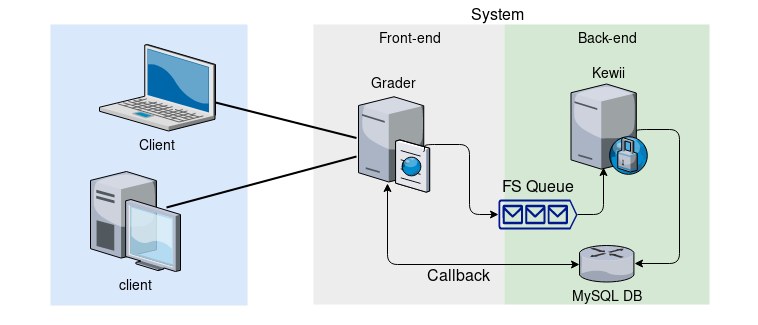
\includegraphics[scale=0.3]{../Figures/graderarchitecture.png}
  \end{figure}
\end{frame}

\begin{frame}
  \frametitle{Έννοιες του συστήματος}

  \begin{itemize}
      \item Προβλήματα
      \item Διαγωνισμοί
      \item Αρχεία Ελέγχου
      \item Διαγωνιζόμενοι
      \item Υποβολές
  \end{itemize}

\end{frame}

\begin{frame}
  \frametitle{Kewii}

  \begin{itemize}
      \item Πρακτικά ο Kewii είναι το σύστημα αυτόματης αξιολόγησης
      \item Τρέχει συνεχώς στο server περιμένοντας υποβολές
      \item Διαθέτει μια ουρά για τις υποβολές και εκτελεί όποια έρχεται σε
        αποκλεισμένο περιβάλλον
      \item Αποτελεί, ουσιαστικά, ένα black box αφού για κάθε υποβολή απλά εκτελεί
        το πρόγραμμα για τα αρχεία ελέγχου που ζητήθηκαν και ενημερώνει τη βάση για
        την επιτυχία/αποτυχία για κάθε αρχείο ελέγχου
      \item Τα υπόλοιπα τα αναλαμβάνει ο Grader
  \end{itemize}
\end{frame}

\begin{frame}
  \frametitle{Ροή Kewii}

  \begin{figure}
    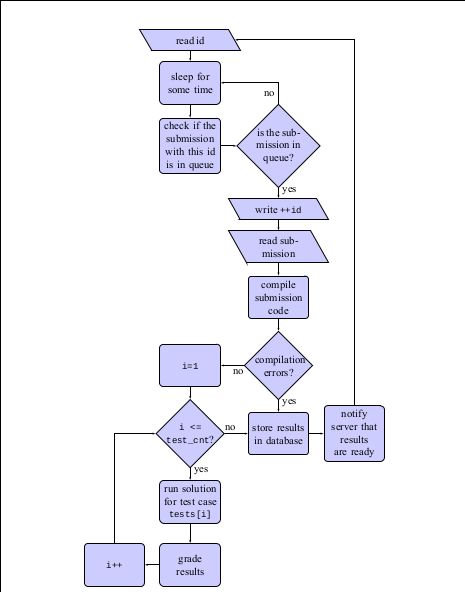
\includegraphics[scale=0.37,trim=4 4 4 4,clip]{../Figures/graderflow.png}
  \end{figure}
\end{frame}

\begin{frame}
  \frametitle{Grader Front-end}

  Το Front-end κομμάτι του Grader αναλαμβάνει τόσο την αλληλεπίδραση με
  διαχειριστές - διαγωνιζόμενους, όσο και την υλοποίηση της συνολικής λογικής
  του συστήματος.

  \bigskip

  Οι λειτουργίες του είναι οι παρακάτω:
  \begin{itemize}
      \item Δημιουργία και διαχείριση διαγωνισμών και προβλημάτων
      \item Ανέβασμα και διαχείριση (ανάθεση πόντων) αρχείων ελέγχου
      \item Υποβολή λύσεων σε ενεργούς διαγωνισμούς από επιλεγμένους διαγωνιζόμενους
      \item Ανάκτηση αποτελεσμάτων υποβολής, αναλυτική παρουσίαση στο χρήστη
      \item Τελική αξιολόγηση και δημοσίευση αποτελεσμάτων
  \end{itemize}
\end{frame}

%todo ισως διαφανεια περιγραφής common workflow

\begin{frame}
  \frametitle{Grader Front-end}

  Το Front-end κομμάτι του Grader αναλαμβάνει τόσο την αλληλεπίδραση με
  διαχειριστές - διαγωνιζόμενους, όσο και την υλοποίηση της συνολικής λογικής
  του συστήματος.

  \bigskip

  Οι λειτουργίες του είναι οι παρακάτω:
  \begin{itemize}
      \item Δημιουργία και διαχείριση διαγωνισμών και προβλημάτων
      \item Ανέβασμα και διαχείριση (ανάθεση πόντων και τύπων εκτέλεσης) αρχείων ελέγχου
      \item Υποβολή λύσεων σε ενεργούς διαγωνισμούς από επιλεγμένους διαγωνιζόμενους
      \item Ανάκτηση αποτελεσμάτων υποβολής, αναλυτική παρουσίαση στο χρήστη
      \item Λήξη διαγωνισμού, τελική αξιολόγηση και δημοσίευση αποτελεσμάτων
  \end{itemize}
\end{frame}

\section{Επεκτάσεις: Testcase Groups}

\begin{frame}
\Huge{\centerline{Επεκτάσεις}}
\end{frame}

%μια διαφανεια blue tag
% prosthiki testcase groups dio logia giati
% pws 8a ginei i ilopoihsh kai pws allazei i logiki
% isws demo
% (3-4) diaf
\begin{frame}
  \frametitle{Testcase Groups και Blue tag}
  Στο πλαίσιο της συγκεκριμένης επέκτασης δημιουργήθηκαν:
  \begin{itemize}
      \item Ένας νέος τύπος εκτέλεσης αρχείων ελέγχου, το Blue tag 
\includegraphics[scale=0.8]{../Figures/tag_blue.png}
      \item Testcase Groups, δηλαδή ομάδες αρχείων ελέγχου
  \end{itemize}
\end{frame}

\begin{frame}
  \frametitle{Τύποι εκτέλεσης αρχείων ελέγχου}
  Τι είναι τύπος εκτέλεσης και ποιοι είναι αυτοί;

  \bigskip

  Οι τύποι εκτέλεσης καθορίζουν το πως και πότε θα χρησιμοποιηθούν τα αρχεία ελέγχου
  στις υποβολές.

  \begin{figure}

    
\includegraphics[scale=0.6,trim=4 4 4 4,clip]{../Figures/tipoi.png}
  \end{figure}
\end{frame}

\begin{frame}
  \frametitle{Blue tag}
  \begin{block}{Λειτουργία τύπου εκτέλεσης Μπλε 
\includegraphics[scale=0.8]{../Figures/tag_blue.png}}
    Οι υποβολές θα ελεγχθούν με το συγκεκριμένο αρχείο ελέγχου την ώρα της υποβολής και ο χρήστης θα μπορεί να δει το αποτέλεσμα, αλλά όχι το αρχείο ελέγχου. Το αποτέλεσμα της εκτέλεσης δεν επηρεάζει το αν θα γίνει δεκτή η υποβολή.
  \end{block}
\end{frame}

\begin{frame}
  \frametitle{Προσθήκη testcase groups}

  Προστέθηκε στον Grader η δυνατότητα δημιουργίας testcase groups, ομάδων
  δηλαδή από αρχεία ελέγχου.

\end{frame}

\begin{frame}
  \frametitle{Testcase groups}

  Τα testcase groups:

  \begin{itemize}
      \item Ανήκουν σε προβλήματα
      \item Αποτελούνται από αρχεία ελέγχου και ένα αρχείο μπορεί να είναι
        σε πολλαπλά groups με διαφορετικό τύπο εκτέλεσης
      \item Έχουν τίτλο και πόντους
      \item Παίρνουν τη θέση των αρχείων ελέγχου ως κύριες μονάδες βαθμολόγησης
  \end{itemize}
\end{frame}

\begin{frame}
  \frametitle{Επεξήγηση Λειτουργίας}

  \begin{itemize}
      \item Αξιολόγηση με βάση groups και όχι tests
      %\item Η αξιολόγηση πλέον σε κανονικές και τελικές υποβολές γίνεται με βάση
      % τα testcase groups που το πρόβλημα περιέχει.
      \item Group σωστό αν αρχεία του σωστά
      %\item Ένα testcase group θεωρείται σωστό και βαθμολογείται μόνο αν έχουν
       % αξιολογηθεί ως σωστά τα αρχεία που περιέχει.
      \item Υποβολή σωστή αν τουλάχιστον ένα group σωστό
      %\item Ως σωστές θεωρούνται οι υποβολές που ικανοποιούν τουλάχιστον ένα group
      \item Απαραίτητα τα groups για κάθε πρόβλημα
      %\item Ο ορισμός testcase groups είναι απαραίτητος για τη λειτουργία της
      % αξιολόγησης σε κάθε πρόβλημα
      \item Script για δημιουργία groups σε όλα τα προβλήματα
      %\item Δημιουργήθηκε script για τη δημιουργία testcase groups για όλα τα
       %υπάρχοντα προβλήματα.
      \item Ο Kewii, ως black box, δεν επηρεάζεται
      %\item Ο Kewii δεν επηρεάζεται, αξιολογεί κάθε υποβολή για τα αρχεία που θα
        %του ζητηθούν. O Grader επιλέγει και φροντίζει κάθε αρχείο να αξιολογείται
        %το πολύ μια φορά, ακόμα κι αν ανήκει σε πολλαπλά groups.
  \end{itemize}
\end{frame}

% todo mhpws diafaneia gia demo
\begin{frame}
  \frametitle{}
  \begin{figure}

    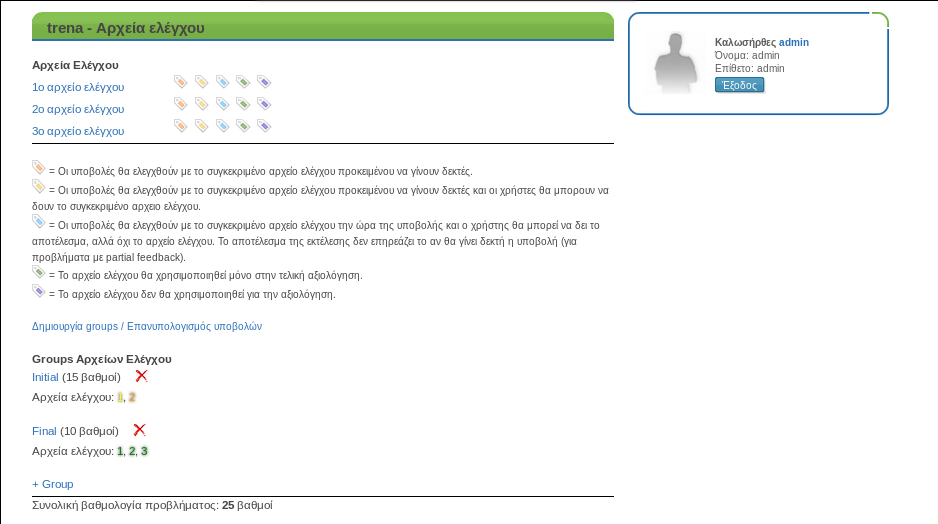
\includegraphics[scale=0.4,trim=4 4 4 4,clip]{../Figures/groupoverview.png}
  \end{figure}
\end{frame}

\begin{frame}
  \frametitle{}
  \begin{figure}

    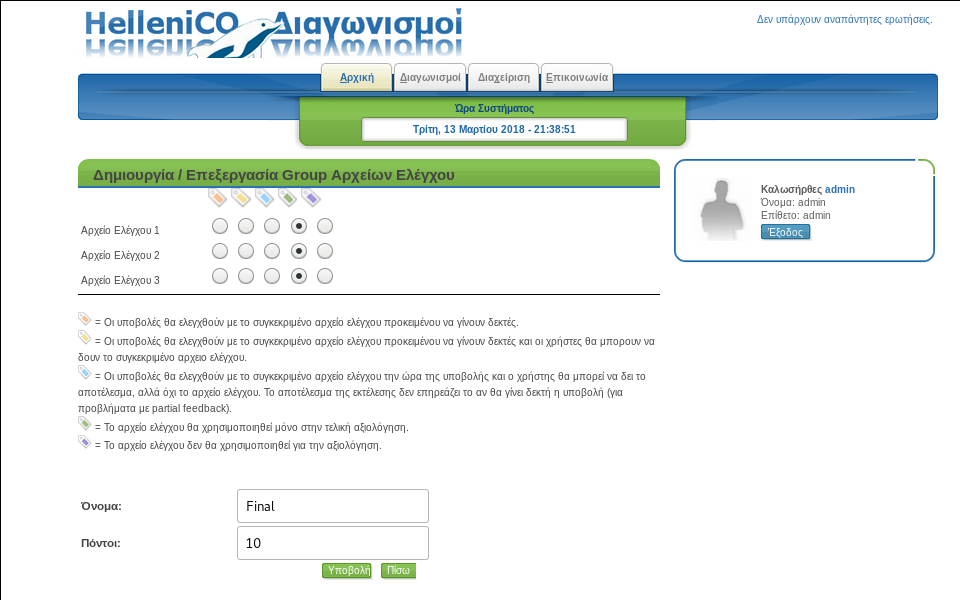
\includegraphics[scale=0.4,trim=4 4 4 4,clip]{../Figures/groupedit.png}
  \end{figure}
\end{frame}

\section{Επεκτάσεις: Αλλαγή σχεδίασης προβλημάτων και διαγωνισμών}
% 2-3 diaf oti eixame 8ema me ti metakinisi kai ti vasi itan etsi egine etsi
% antigrafi provlimatos kai epanaxrisimopoihsh
\begin{frame}
  \frametitle{Αλλαγή σχεδίασης προβλημάτων και διαγωνισμών}

  Στην αρχική σχεδίαση του Grader δεν είχε προβλεφθεί η ύπαρξη προβλήμάτων
  σε πολλαπλούς διαγωνισμούς. \\[0.3cm]

  Επιτρέπεται όμως η μετακίνηση ενός προβλήματος σε άλλο διαγωνισμό. \\[0.3cm]

  Αυτό αρκεί για την επαναχρησιμοποίηση προβλημάτων αλλά δημιουργεί επιπλοκές.

\end{frame}

\begin{frame}
  \frametitle{Επιπλοκές μεταφοράς προβλημάτων}
  
  \begin{itemize}
      \item Ανεπιθύμητη μεταφορά υποβολών
      \item Παλαιότεροι διαγωνισμοί χωρίς προβλήματα
  \end{itemize}% \\[0.3cm]

  \bigskip

  Πώς επιλύονται αυτές οι επιπλοκές;
\end{frame}

\begin{frame}
  \frametitle{Αλλαγές στη βάση: Πριν}
  

  \begin{figure}

    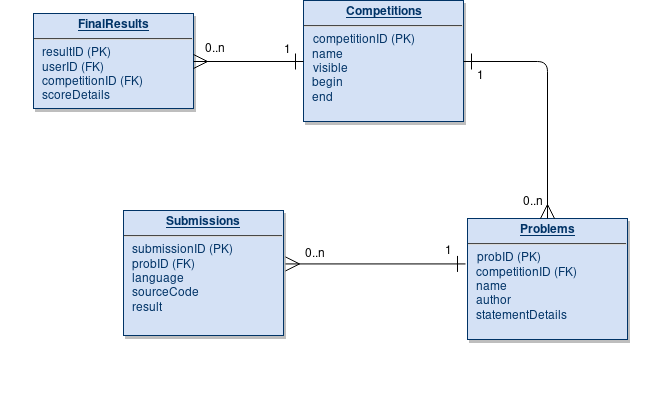
\includegraphics[scale=0.4,trim=4 4 4 4,clip]{../Figures/sepbefore.png}
  \end{figure}
  
\end{frame}

\begin{frame}
  \frametitle{Αλλαγές στη βάση: Μετά}

  \begin{figure}
    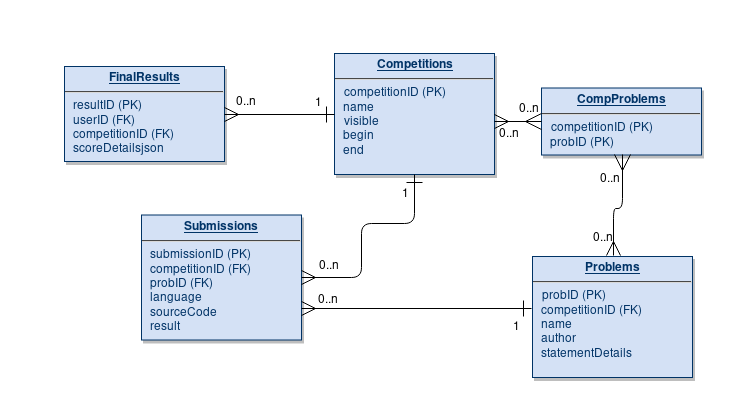
\includegraphics[scale=0.4,trim=4 4 4 4,clip]{../Figures/sepafter.png}
  \end{figure}
  
\end{frame}

\begin{frame}
  \frametitle{Προσθήκη λειτουργικότητας αντιγραφής προβλήματος}

  Η αλλαγή της βάσης επιτρέπει την ύπαρξη των προβλημάτων σε πολλαπλούς διαγωνισμούς
  με ξεχωριστές υποβολές. \\[0.3cm]
  
  Δεδομένου ότι δεν υπήρχε πλέον λόγος για μετακίνηση προβλημάτων, προστέθηκε η
  δυνατότητα αντιγραφής αυτών σε άλλους διαγωνισμούς.
\end{frame}

\section{Επεκτάσεις: Python, Mass Testcase Upload, Connector PDO}
% mia diaf gia python 2 kai poies itan, python 3 soon
% automato anevasma testcases + groups, descriptor, anafora sto ergaleio isws demo
% mia diafaneia pdo asfaleia prepared statement abstraction
\begin{frame}
  Λαλαλα σαδλασδ αλδλςαδλςα
  \begin{itemize}
      \item asdas
      \item σδασδασ sadaw
  \end{itemize}
\end{frame}


\section{Μελλοντική Εργασία}
% mia diafaneia me ena itemize me oles tis malakioules
\begin{frame}
  Λαλαλα σαδλασδ αλδλςαδλςα
  \begin{itemize}
      \item asdas
      \item σδασδασ sadaw
  \end{itemize}
\end{frame}

\begin{frame}
  \frametitle{Τέλος}
  \centering
  Ευχαριστώ!
\end{frame}

\begin{frame}
  \frametitle{Τέλος}
  \centering
  Ερωτήσεις;
\end{frame}

\end{document}
